\title{GEC Models}
\documentclass[12pt, letterpaper, onecolumn, oneside]{article}
\usepackage{amsmath, graphicx, natbib}
\linespread{1.3} %Line spacing
\oddsidemargin -0.5in %Creates 1 inch margins all around
\textwidth 7.5in
\topmargin 0in
\headheight 0in
\headsep 0in
\textheight 9in
\begin{document}
%\maketitle

\section*{Notes and Intro}

This is a list of various plausible sources of the global electric circuit (GEC) with their accompanying references. When possible variables and estimates used will be listed for usage in a WWLLN derived GEC source estimate. Maybe a table will be created at the end as a reference.

%\subsubsection*{Campaign Names}
%\begin{itemize}
%\item{{\bf GEC} - Global Electric Circuit}
%\item{{\bf FW} - Fair Weather}
%\item{{\bf RC} - Return Current}
%\item{{\bf C} - Concurrent, Campaign}
%\item{{\bf O} - Observations}
%\item{{\bf S} - Simultaneous}
%\item{{\bf B} - Balloon}
%\item{{\bf HA} - High-Altitude}
%\end{itemize}
%
%{\bf GECCO} Global Electric Circuit Concurrent Observations

\section*{GEC Sources}

Check {\bf\citep{Roble1991}} (from \citet{Siingh2007})

\subsection*{Thunderstorms}

200 thunderstorms are active at one time, concentrated over the tropical landmasses and cover 10\% of the Earth's surface {\bf\citep{Markson1978}}. (\citep{Siingh2007}).

Maxwell current from {\bf\citet{Ruhnke1969}} as source as it varies slowly through the evolution of the storm and is fairly independent from impulsive events like lightning (\citep{Siingh2007}).

Electrified clouds - {\bf\citep{Rycroft2008}}

\subsection*{Lightning}

Whistlers impact the GEC due to precipitation particles lowing the ionospheric potential {\bf\citep{Rycroft1991}} (\citep{Siingh2007}).

\subsection*{Transient Luminous Events}

Large perturbations and charge moved from transient luminous events, such as gigantic jets moving 30C of charge, need to know their frequency {\bf\citep{Pasko2003}} (\citep{Siingh2007}).

A TLE has been seen to enhance conducitivity above a thunderstorm by a factor of 2 {\bf\citep{Holzworth1995}} (\citep{Siingh2007}).

However TLE's are all on the upward branch of thunderstorms while the source of the GEC should be in in the downward branch \citep{Rycroft2000c} \citep{Siingh2007}.

\subsection*{Schumann Resonances}

Since the source of Schumann resonances are lightning and sprite activity and it varies fairly closely to global lightning it should track with ionospheric potential, with any variability due to non-thunderstorm sources \citep{Siingh2007}. Based on this I should see about making an SR measurements along with the WWLLN and Balloon measurements to have a back-up, also it SR should only track with lightning and not thunderstorms.

\subsection*{Ionospheric Dynamo}

Tidal wind system drives ionospheric plasma against the geomagnetic field to produce large horizontal currents, the $S_q$ current system. They give rise to the equatorial electrojet. No evidence that the dynamo effects the GEC. \citep{Siingh2007}.

\subsection*{Magnetospheric Dynamo}

It is there and may impact conductivity in auroral regions during geomagnetic storms \citep{Siingh2007}.

\section*{GEC Models}

\subsection*{Mathematical Models}

From \citep{Siingh2007} check out {\bf\citep{Hill1971, Roble1991}}.

\subsubsection*{\citet{Hays1979}}

\citet{Hays1979} have a quasi-static model with thunderstorms as current sources, include orography, and coupling along geomagnetic field lines. Did not account for geospatial height variations of the conductivity. \citet{Makino1984} made a similar model but omitted aerosol particle concentration near the earth surface. (\citep{Siingh2007}).

\subsubsection{\citet{Kasemir1977}}

\citet{Kasemir1977} uses a novel model in which he sets infinity at 0V and treats the ionosphere as increasing to infinity. They state that this allows the source and return current to be treated separately and allows for other generators to be easily added in. It also does not assume an equipotential layer in the ionosphere. He solves the system in terms of Henkel functions and Legendre polynomials (instead of spherical harmonics).

They go through how they model things such as columnar resistance, global resistance and the like. They keep mentioning the austausch layer, which I believe is the layer nearest the ground which has laminar flow and heat exchange.

This paper was cited as having a quantitative analysis of the thunderstorm size to current output relation, however after reading it I did not see any discussion of such a relationship. They only mention is that they assume all thunderstorms act as a point source since their area is so much less then the surface area of the earth. (I read the wrong article, this is not \citet{Vonnegut1963} but \citet{Kasemir1977}).

\subsection*{Aerosol Models}

{\bf\citet{Sapkota1990} }looked at pollution from aerosol particle ionization, solar activity and stratospheric aerosol particles effects on the GEC. Increased stratospheric aerosol particles increases the global resistance and decreases the global current and ionospheric potential. (\citep{Siingh2007}).

\subsection*{Circuit/Engineering Models}

\subsubsection*{\citet{Ogawa1985}}

\citet{Ogawa1985}: uses the model of {\bf \citet{Holzer1952}} for the amount of current flowing out of a thunderstorm, using some basic physics and some assumptions about charge center heights and the conductivity profile arrives at a ratio of current flowing to the ionosphere $I_u$ to convection supply current $I_o$ of:

\begin{equation}
I_u=\frac{q_1}{\epsilon_o}\sigma_o\frac{exp\{(z_1-z_o)/\alpha\}-1}{1-exp(-h/\alpha}
\end{equation}

\begin{equation}
\frac{I_u}{I_o}=exp(-z_o/\alpha)-exp(-z_1/\alpha)
\end{equation}

where $q_o, z_o$ correspond to the lower charge layer and $q_1,z_1$ correspond to the upper charge layer.

He concludes that the largest controller is cloud top height, so clouds near the equator are larger contributors then those at mid-latitudes. 

It is mentioned that a CG discharge will upset the assumptions and increase the total upward current $I_u$. Also this is all for a point thunderstorm and not a distributed storm.

From \citet{Makino1984} it is seen that $J_z$ varies by 20\% due elevation (0-9000km) and -20\% due to latitude.

Now to turn to the work done by \citet{Rycroft2000c}, first there is a pretty good introduction to the problem and the GEC in this paper. He throws out the number of 1000 thunderstorms globally, so that makes the estimated range 200-2000. He lists the current flowing upward from a thundercloud to be 0.1 to 6 A with an average of 0.5 to 1 A per thunderstorm cell {\bf \citep{Blakeslee1989}}.

To estimate the ionospheric charge think of the current output from thunderstorms going through a charging resistor of the ionosphere, estimated at $10^5$-$10^6 \Sigma$. The ionosphere is not constant with several altering factors:

\begin{itemize}
\item{Dawn-to-dusk potential difference ~100kV}
\item{Auroral/magnetospheric processes ~100kV}
\item{Unipolar induction from the rotating geomagnetic field ~91 kV at equator with respect to pole}
\item{Dynamo action ($S_q$) ~20kV}
\end{itemize}

The conductivity between the thunderstorm and ground can be effected by point discharges in updraughts, CG strokes and altitude above sea level.

There are a bunch of estimates for various components of the GEC, but there is little justification for any of them.

St. Elmo's fire, point discharges, may be the source of up to half of the GEC, see {\bf \citet{BeringIII1998}}.

There is some qualitative stuff about solar influences and aerosols.

It is unknown (as of this paper) if sprites contribute to the GEC or if they do by how much. They are estimated to occur for 1 in 200 lightning strokes.
 
All of this is put together based on some work by \citet{Hays1979} to give a global circuit model. They solve the system in spherical harmonics to arrive at each thunderstorm giving a potential of 36V to the ionosphere. Too low based on 2000 thunderstorms and assumes uniform thunderstorms.

\subsubsection*{\citet{Hays1979}}

\citet{Hays1979} starts by listing all of the important components to considering in a GEC model:

\begin{itemize}
\item{Orography}
\item{Magnetic field lines and anisotropic conductivity}
\item{Ionospheric current systems}
\item{Geospatial variation in conductivity and columnar resistance}
\item{Lower atmosphere generators such as thunderstorms and convection}
\end{itemize}

Like all models they assume there are 2000 point thunderstorms around the globe with little to no substantive evidence that there are so many thunderstorms. The model is very similar to the other mathematical models.

\subsubsection*{\citet{Rycroft2000c}}

\citet{Rycroft2000c} kept the passive elements but had three different regions for the $J_z$. He also throws in a lot of numbers for assumptions which leads to the conclusion that sprites and other transients will have little effect on the GEC. This model was updated with new generators in {\citet{Rycroft2006}. (\citep{Siingh2007}).

\subsubsection*{\citet{Rycroft2006}}

\citet{Rycroft2006} mentions a numerical model of ionospheric potential distribution in relation to thunderstorms by \citet{Kartalev2004}. But in this paper they use a spherical shell model to make a 3d model.

He says that there are currently (as of ~2005) no methods of translating lightning intensity distributions to current densities above thunderstorms. Along this line he mentions \citet{Holzworth1981, Makino1984} for measurements and estimates of currents above thunderstorms. Could this be something that I need to do? From these he gets a maximum upward current of $70 x 10^{-6}$ A/km$^2$ with an average of $40 x 10^{-6}$ A/km$^2$.

\subsubsection*{\citet{Kartalev2004}}

They modeled the distribution of potential in the ionosphere, not much use.

\subsubsection*{\citet{Makino1984}}

\citet{Makino1984} has details on a latitudinally dependent conductivity model of the ionosphere. They then model the distribution of thunderstorm charge heights based on the works of \citet{Pierce1970} {\bf \citet{Ogawa1969, Prentice1977, Ogawa1982}}. Interestingly the altitude of the earth's surface just went into the conductivity modeling and not into the thunderstorm current model.

Thunderstorm current source is assumed to be distributed based on maps/work from \citet{Turman1982, Brooks1925}. This is taken in with the charge heights to get at the effective resistance of the thunderstorm column. Then they assume a gaussian of activity centered at 16 LT for each region (WWLLN can fix this). Then they sum over each current source/grid to get the global current source. They also fold in the ionospheric conductivity map to get the total current and charge on the ionosphere. The charged ionosphere is then fed through the resistance map again to give the fair weather current. So far one of the more reasonable models I have read about.

The work by \citet{Turman1982} was preliminary global lightning distribution done on a military satellite.

If the thunderstorms are treated as current sources then any change in the ionospheric conductivity will change the ionospheric potential and from there $J_z$. They reference {\bf \citet{Willet1979}} for a discussion on why treating them as current generators is better then as voltage generators.

Something about {\bf\citet{Harrison2005}}.

\subsection*{Other Model Considerations}

\subsubsection*{\citet{Siingh2007}}

\citet{Siingh2007} suggests to consider the Maxwell current generated from sferics and other radiation in the EIWG since for different frequencies the waveguide can act as a dielectric or a conductor. They refer to {\bf\citet{Singh2004}} for more on the Maxwell current. They also point out that TLEs change the properties of the medium and columnar resistance should be considered.

\subsubsection*{\citet{Makino1984}}

\citet{Makino1984} and another (I forget who) mention that models tend to either treat the ionosphere as an equipotential or treat the geomagnetic field lines as equipotential. Not sure if I need to go into that or not.

\section*{Relating WWLLN}

\subsubsection*{\citet{Holzworth1981}}

Based on \citet{Holzworth1981} the current density over thunderstorms ranges from 10-40 pA/m$^2$. If we found more measurements of the current density perhaps we could see about making a relation between lightning power to thunderstorm output which is then multiplied by that thunderstorms area. 

\subsubsection*{\citet{Blakeslee1989}}

\citet{Blakeslee1989} is a survey of electric fields and currents from flights over a collection of thunderstorms. They found that conductivity did not correlate well to when they were over thunderstorms, in disagreement with measurements from \citet{Holzworth1986a}. See that the current above thunderstorms is relatively independent of the cloud electric field (lightning).

At the ground the current is dominated by the displacement current while at overflight altitudes more then half is from the Maxwell current density with displacement current still providing a healthy amount of the total. They call total integrated current above the storms the storm current (some assumptions in this).

They found that storm current ($J_m$) estimates are linear with storm flash rate from 0.09 to 5.9 A with an average of 2.2 A, figure~\ref{Blake1}. This implies that charge transfer per flash should be independent of the storm characteristics or flash rate. \citet{Koshak1989} showed that the charge transfer did not vary between large and small storms (check this for flash to storm characteristics). This is all contrary to a supposed fifth power dependence between flash rate and cloud size of \citet{Williams1985}.

\begin{figure}[ht!]
   \centering
   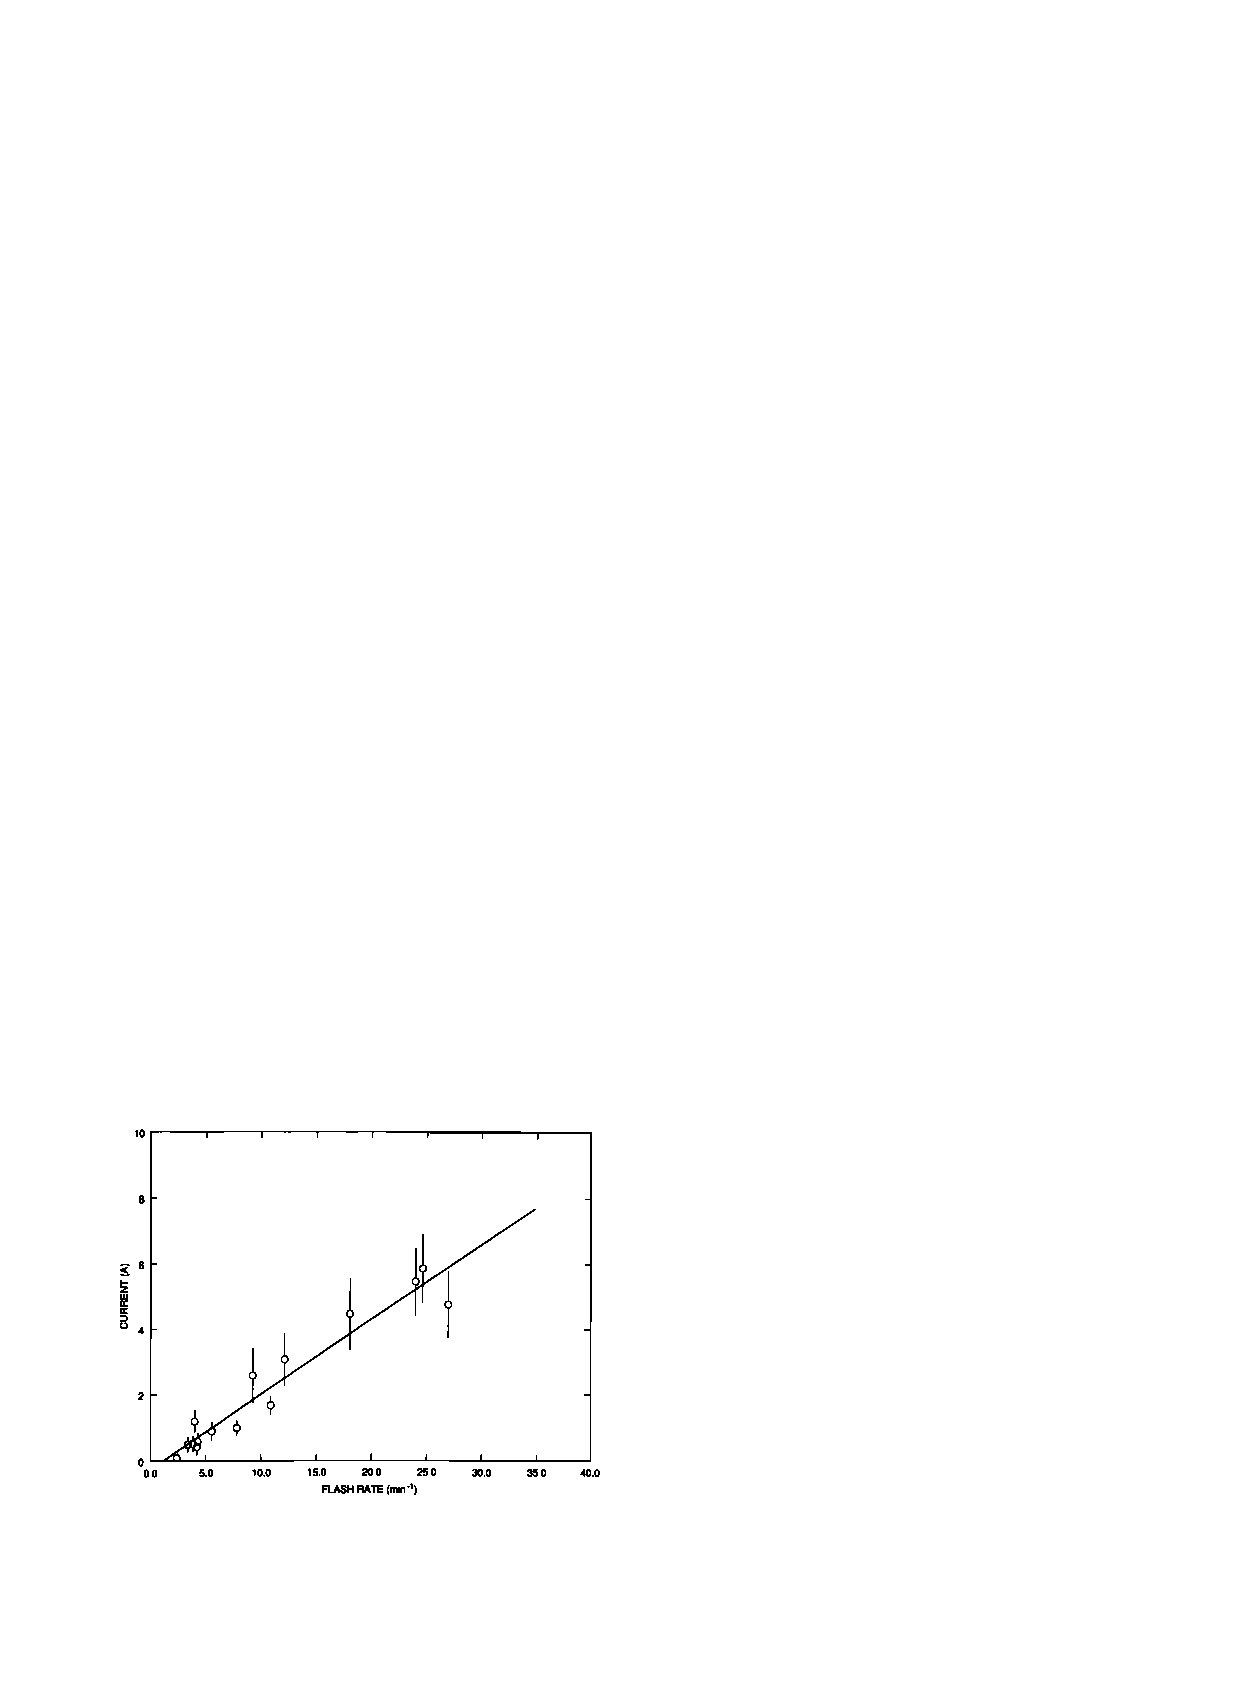
\includegraphics[scale=1]{Blake1.pdf} 
   \caption{"Area integrated $J_m$ versus lightning flash rate for 15 COHMEX storm traverses. The integration of $J_m$ neglects that portion of the signal directly associated with lightning discharges. The errors bars correspond to the standard deviation" \citep{Blakeslee1989}.}
   \label{Blake1}
\end{figure}

The Wilson Current ($I_c$, just conduction) represents more closely a storms contribution to the global circuit and it varied from 0.09 to 3.7 A with an average of 1.8 A, figure~\ref{Blake2}. This falls in with past observations by \citet{Gish1950, Stergis1957}. $I_c$ does not vary linearly with flash rate, it levels off at 3.5A and so the efficiency of a storm to add to the global circuit may be inversely related to flash rate.

\begin{figure}[ht!]
   \centering
   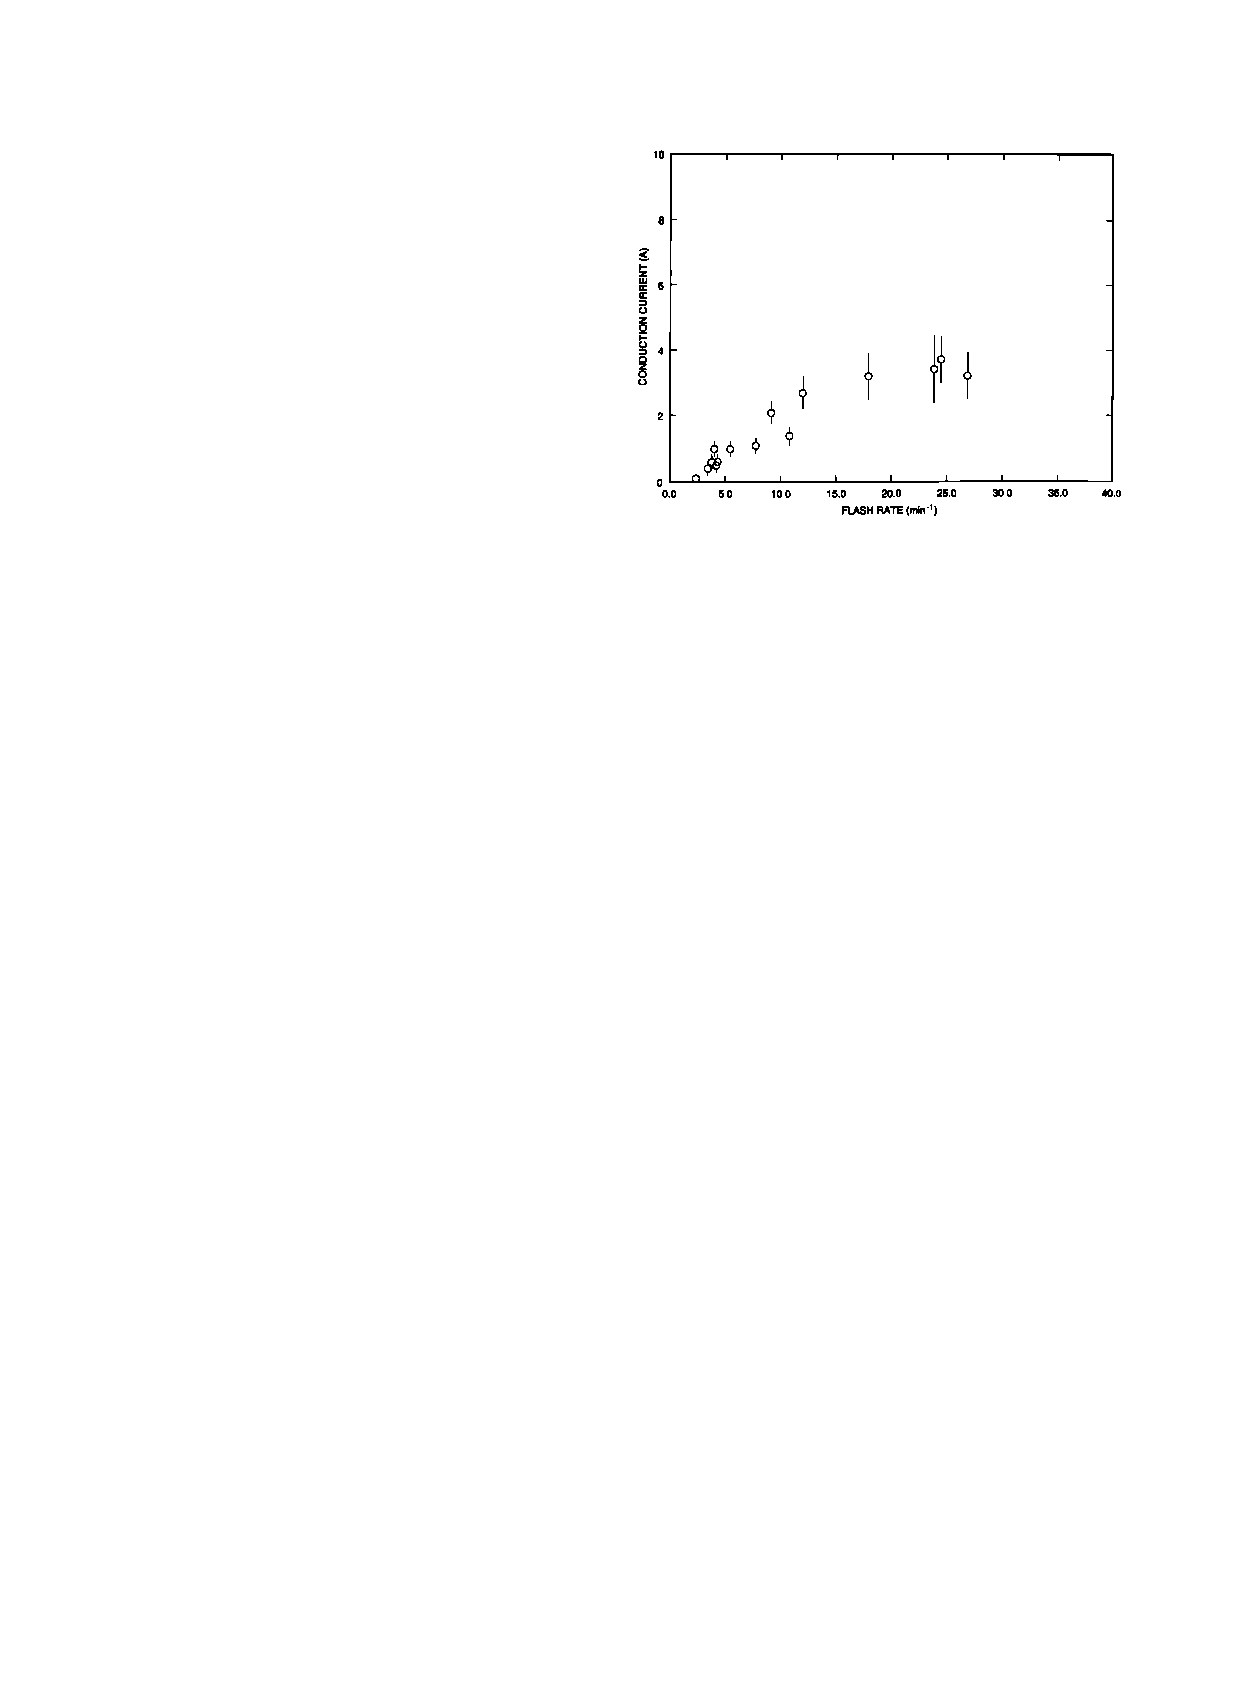
\includegraphics[scale=1]{Blake2.pdf} 
   \caption{"Wilson conduction current (i.e. area-integrated $J_c$) versus lightning flash rate for 15 COHMEX storm traverses. The error bars correspond to the standard deviation" \citep{Blakeslee1989}.}
   \label{Blake2}
\end{figure}

This all implies that the charge separation processes in clouds are split between adding to discharges or adding to the conduction current. {\bf \citet{Schonland1953}} notes something similar in that a large portion of the charging energy goes to maintaining to dipolar field of the thunderstorm.

It is noted that these results may not be universally applicable to all types of storms. Ideally I would have access to a lot of travel money and a well equipped UAV to fly over storms around the world.

\subsubsection*{\citet{Williams1985}}

\citet{Williams1985} addresses the relationship betwween flash rate and size. Mentions that \citet{Vonnegut1963} has a semiquantitative assessment of the electrical output of thunderstorms related to their size.

He says that the flash rate is related to the fifth power of the cloud height/width. Also he claims that flash rate appears to be a true measure of the quasi-steady state electrical power produced by the thunderstorms. So the energy (power) per flash must be independent of the size of the thunderstorm. It is stated that a storm with 10 times the flash rate of another should only have 3 times the cloud charging current. His scaling laws:

\begin{align}
\nabla \cdot E = \rho / \epsilon + E - \rho L - L \\
V = \int E \cdot dl - \rho L^2 - L^2 \\
I = J \cdot (area) - \rho v L^2 - v L^2 \\
P = I \cdot V - v L^2 \cdot L^2 - v L^4
\end{align}

where $v$ is the air velocity and $L$ is the storm thickness/width. It is shown in the paper that air velocity scales with cloud size linearly. Flash rate is also shown to scale with cloud height to the fifth power. And if height is a large controller of contribution to the GEC (see other references who say this) then the flash rate is a (almost) direct indicator of a storms contribution to the GEC. However height, conductivity and orography will still need to be accounted for to calculate the charging resistor above each storm for the ionospheric potential.

Here are the plots he used to show the relation between air velocity and cloud size (figure~\ref{Williams1}) and flash rate and cloud height (figure~\ref{Williams2} and~\ref{Williams3})

\begin{figure}[ht!]
   \centering
   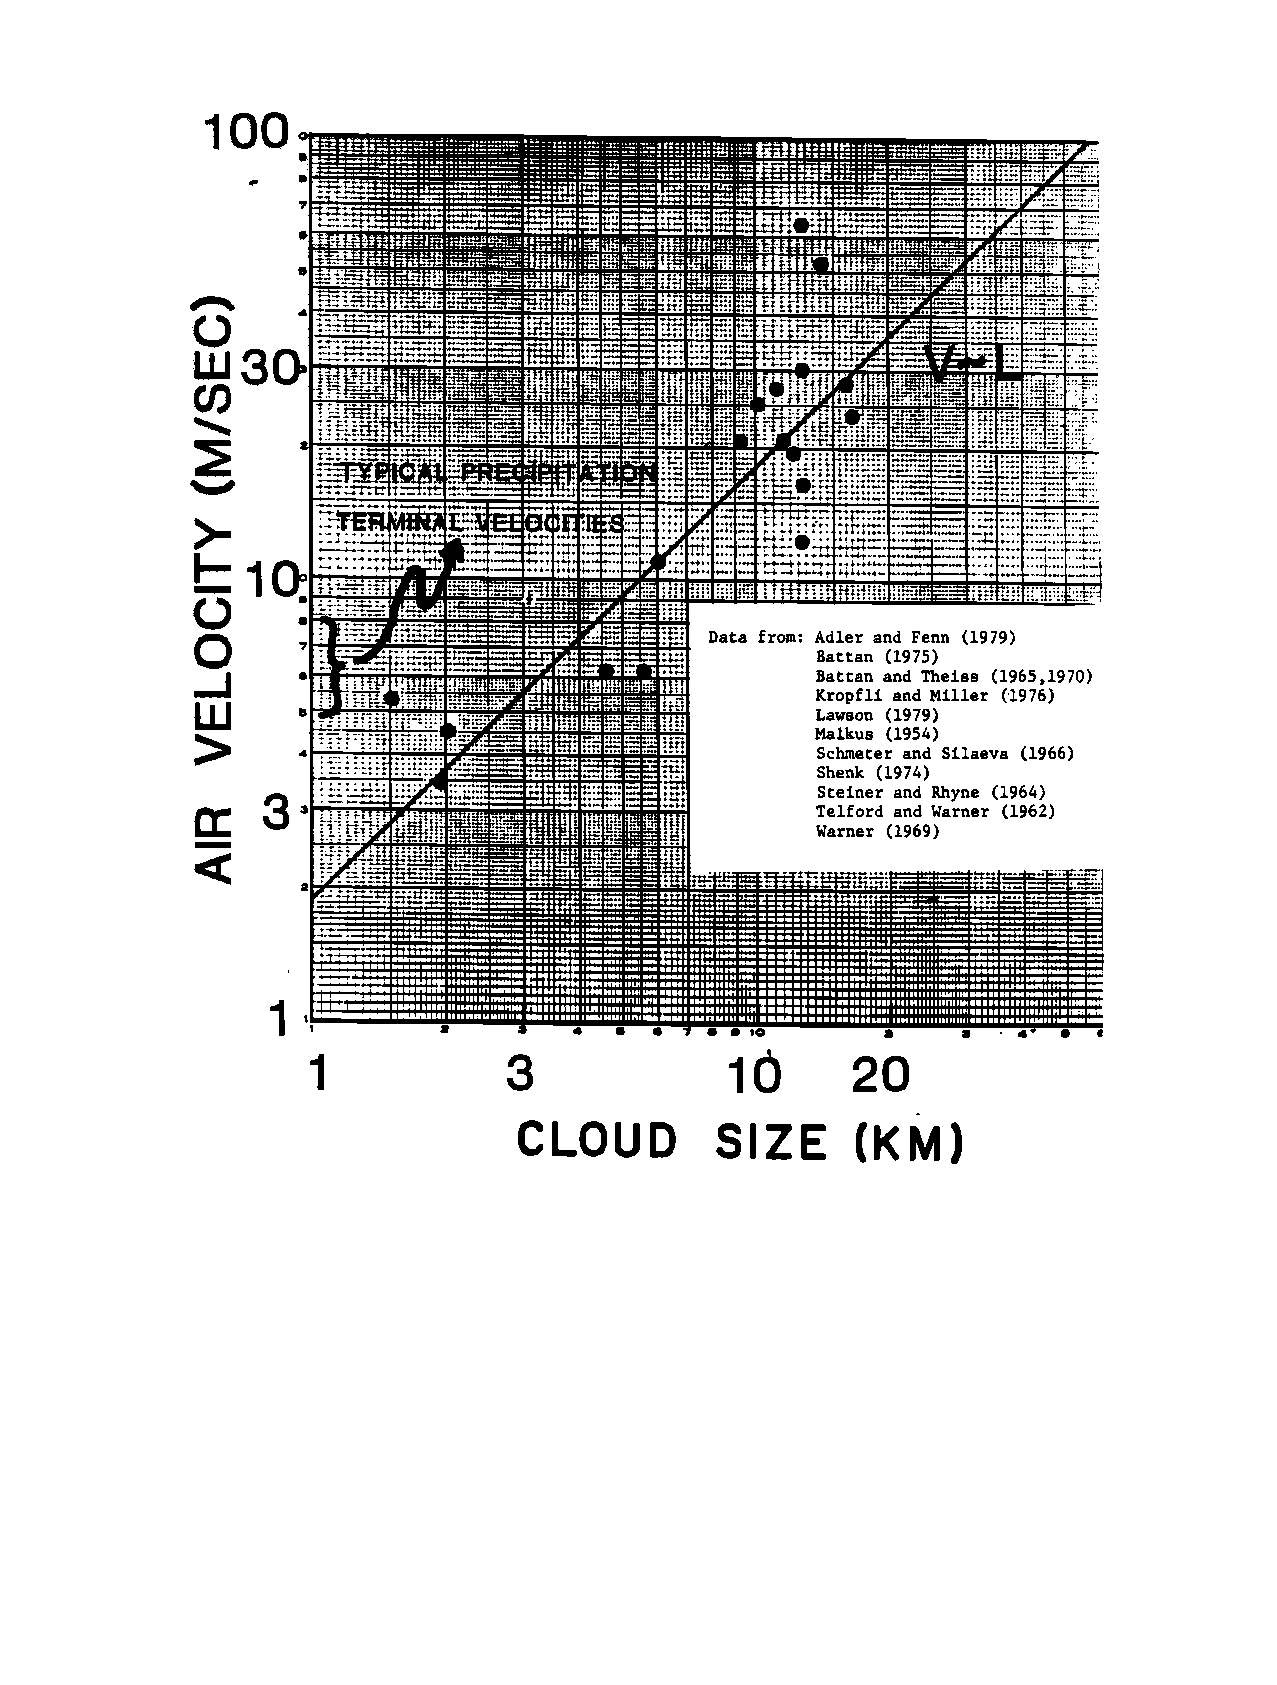
\includegraphics[scale=.75]{Williams1.pdf} 
   \caption{``Compilation of maximum vertical air motion in clouds of various sizes, illustrating empirical increase of convective velocity with cloud size" \citep{Williams1985}.}
   \label{Williams1}
\end{figure}

\begin{figure}[ht!]
   \centering
   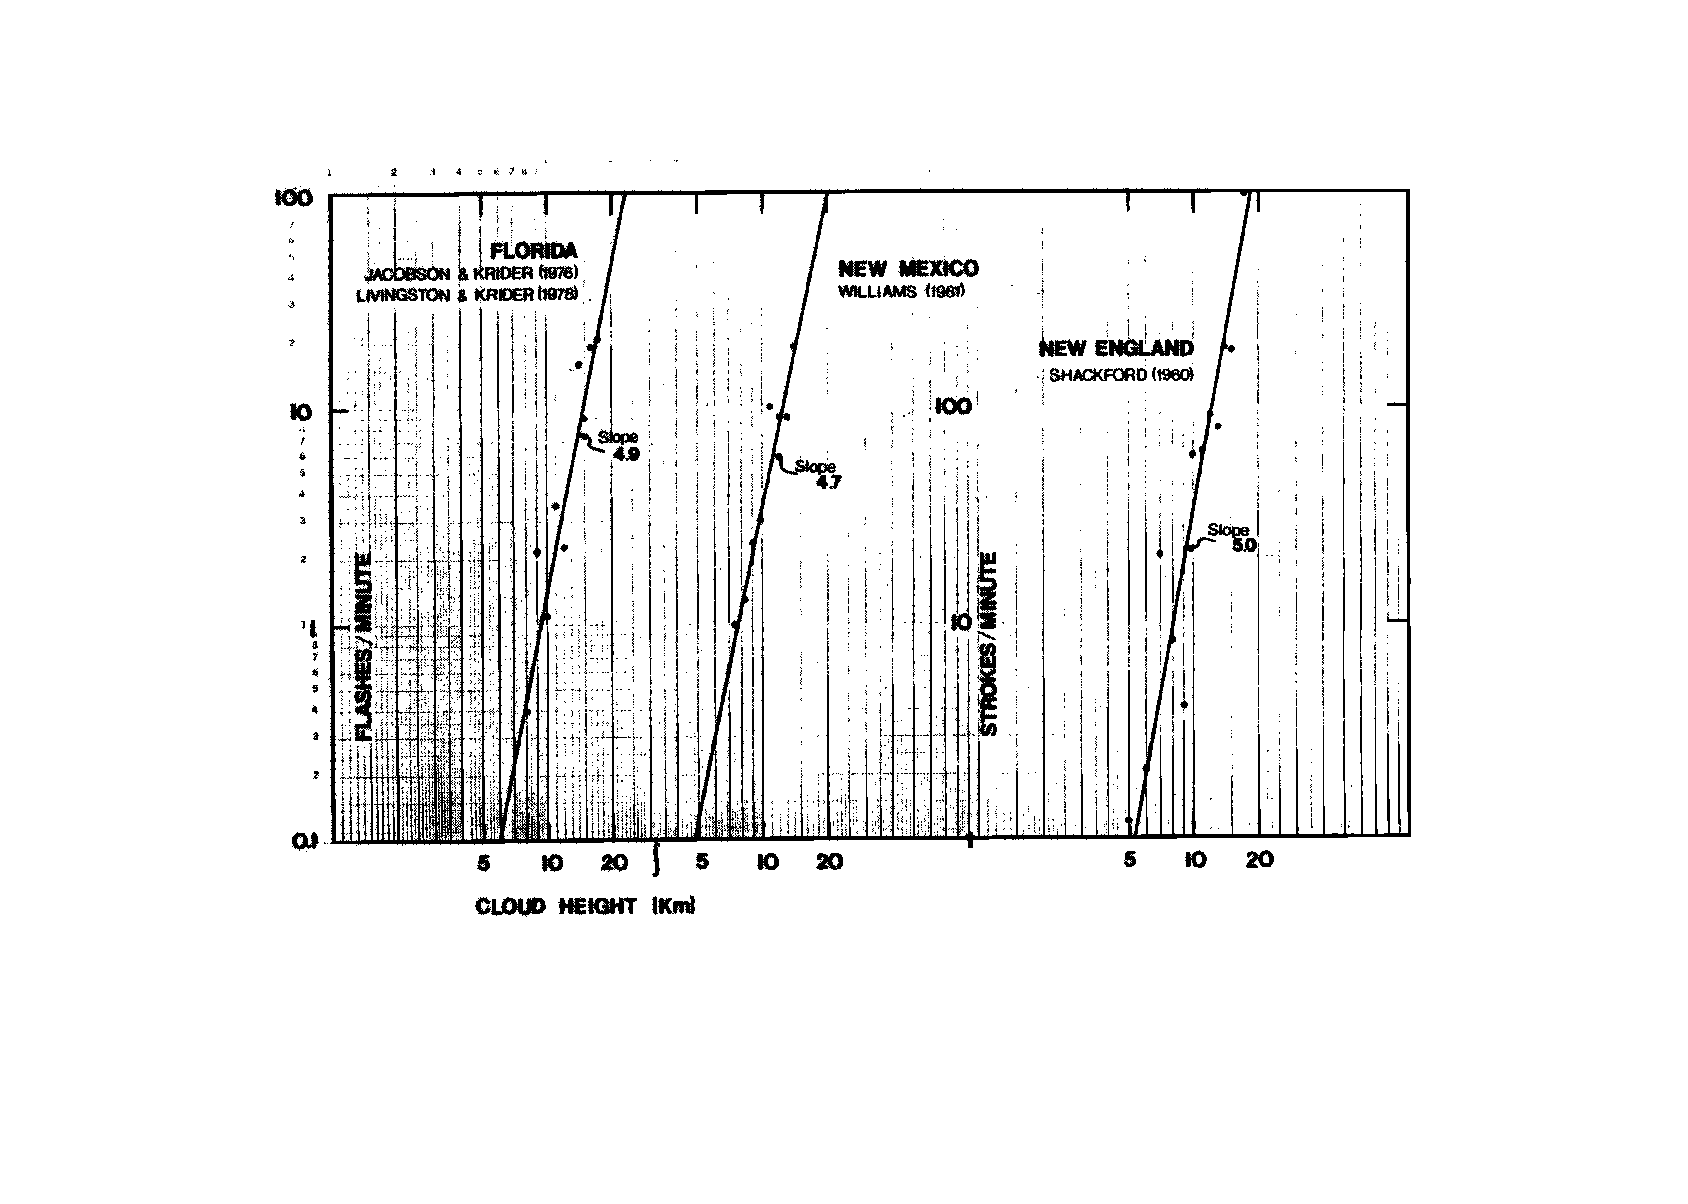
\includegraphics[scale=.9]{Williams2.pdf} 
   \caption{``Experimental tests of scaling law prediction: data on flash rate versus cloud height for storms in Florida (source), New Mexico (source) and New England (source)" \citep{Williams1985}.}
   \label{Williams2}
\end{figure}

\begin{figure}[ht!]
   \centering
   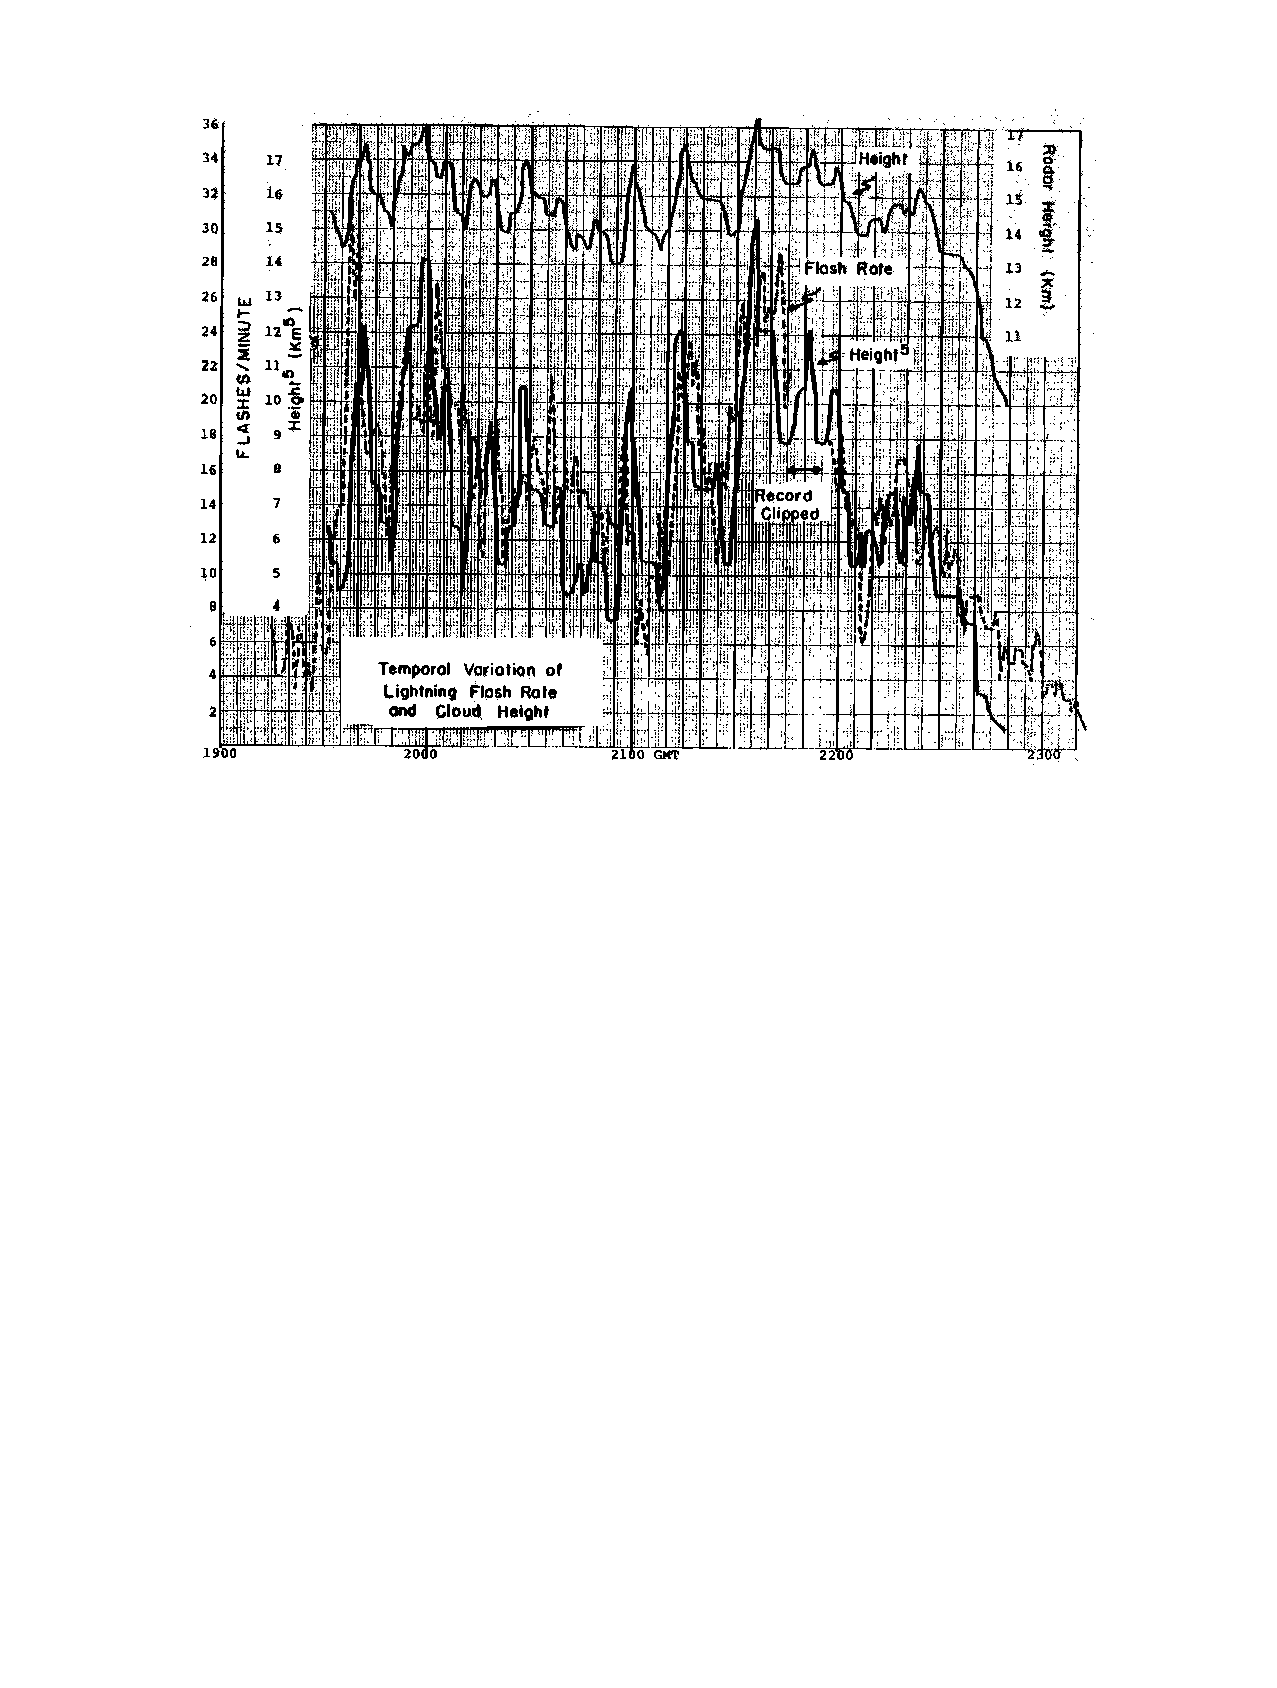
\includegraphics[scale=.75]{Williams3.pdf} 
   \caption{``Temporal variation of lightning flash rate, cloud height, and fifth power of cloud height for for August 10, 1976, Florida thunderstorm (source)" \citep{Williams1985}.}
   \label{Williams3}
\end{figure}

\subsubsection*{\citet{Vonnegut1963}}

\citet{Vonnegut1963} makes a basic argument that the energy between two charged spheres varies as $R^5$ and so the energy available per unit length of cloud spark (i.e. lightning) should vary as $R^4$, and points out that strokes are rare for small clouds. Similarly the rate of electrical power generation varies as $R^5$. Here is the basics of the electrostatic arguments:

Consider a sphere of radius $R$ and charge density $\rho$, the energy stored in the sphere is then:

\begin{equation}
J=\frac{16}{15}\pi^2 \rho^2 R^2
\end{equation}

Then we assume there are two tangential spheres with the same radius and density the energy becomes:

\begin{equation}
J=\frac{56}{45} \pi^2 \rho^2 R^5
\end{equation}

And so if we assume that the size of the charge region is proportional to the size of the cloud then it follows that the energy available for a length of spark goes as $R^4$. Assuming a velocity and air transport $v$ we get a conduction current:

\begin{equation}
I = \pi R^2 \rho v
\end{equation}

And the power generated:

\begin{equation}
W=\frac{8}{3}\pi^2 \rho^2 K^2 R^4 v
\end{equation}

Where $K$ is the ratio between the charge centers and size of the storm. Depending on how $v$ is related to $R$ we get the result that the electrical power generated could go as $R^4$ or $R^5$.

\subsubsection*{\citet{Koshak1989}}

\citet{Koshak1989} analyzes field mill data around Cape Canaveral. Describes storm phases as having a high flash rate active phase, followed by the end-of-storm oscillation which is characterized by a lower flash rate, larger electric fields and large field changes \citep{Livingston1978}.

Some time is spent discussing how the field mill data was analyzed for active storms and how it had to be improved in order to get at the background field when saturated with strokes.

They are saying that the electric field/charge deposited per stroke is independent of thunderstorm size, contrary to the results of  \citep{Williams1985}, say this could be due to their small statistics.

Mentions that this work should be combined with others on discharge evolution, storm information, and (importantly to me) evolution and pattern of the Maxwell current density in \citet{Krider1985, Krider1982}}.

\subsubsection*{\citet{Livingston1978}}

\citet{Livingston1978} used the same setup as \citet{Koshak1989} with 25 thunderstorms over Cape Canaveral. Larger storms lasted 3 hours with smaller storms about 1 hour. Lots of tables and plots with storm averages and information about the active phase of storms. Nothing empirical but state that flash rate should be related to lightning currents and conduction currents should be related to storm area. So another reference in favor of storm size related to GEC.

\subsubsection*{\citet{Gish1950}}

\citet{Gish1950} used data from 21 thunderstorm overflights (Mid-west), they estimate total current that range from 0 - 6.5 A with the average of 0.8 A (0.5 A without the largest). Finally! They say that the estimate of 2000 thunderstorms is based on an observed return current of 1kA and an average storm current of 0.5 A ($J_z=N\cdot I$).

They observed that the conductivity over a storm at higher altitude (30,000 ft) is the same over or far away from a storm.

\subsubsection*{\citet{Holzworth1986a}}

\citet{Holzworth1986a} shows the opposite of \citet{Gish1950} in reference to the conductivity over thunderstorms. The balloon overflights show that conductivity is quite evident of thunderstorms with a change in factor of 2. These changes of conductivity could have effects of 10-30\% over assuming the same conductivity profile of fair-weather.

\subsubsection*{\citet{Stergis1957}}

\citet{Stergis1957} see that conductivity remains the same over and away from thunderstorms during 25 balloon overflights over Florida. They found a current range of 0.6 - 4.3 A with an average of 1.3 A. They assumed, like everyone else, cylindrical symmetry for their overflights. They mention that these numbers are likely the lower current bounds and may be off by as much as 50\%. They also come to the same conclusion of many, that light strokes are not the actual drivers of the current.

\subsubsection*{\citet{Krider1985}}

\citet{Krider1985} looked at Maxwell currents below a thunderstorm using a similar KSC network as \citet{Livingston1978, Koshak1989}. They see that $J_m$ is steady with abrupt, but insignificant, changes due to lightning.

\subsubsection*{\citet{Tonev2007}}

\citet{Tonev2007} mentions past modeling papers as past studies of currents above the ionosphere. In the work they look at how the peak quasi-static fields above a thunderstorm vary with the charge moment change, horizontal scale, lightning discharge time, and the conductivity profile. Says that \citet{Fullekrug2004} shows that a CG stroke has significant effect on the GEC, contrary to other examined works.

They develop a 2D model for the fields and currents. They explain their assumptions and equations to get at something solved with Bessel functions. They say that the current output, both Maxwell and Conduction, are linearly related to the charge moment change of the thunderstorm and the peak values are linearly related as well. Their arguments are not very persuasive or convincing.

\subsection*{Lightning Scaling}

Check it: {\bf \citep{Markson1978, Allen2002, Solomon1998, Cherna1986, Futyan2007}}

\subsubsection*{\citet{Ushio2001}}

\citet{Ushio2001} continues with the work of \citet{Williams1985, Vonnegut1963} using TRIMM and LIS. They are looking at instaneous cloud top heights with the flash rate over at most 83 seconds of view time. They find the 5th power relationship to hold over Florida during the same season that \citet{Williams1985} used. They find that different regions (latitude bands) have different functions ranging from 4th to slightly above 5th power relationships, all with different coefficients, their results are compiled in table~\ref{Ushio}. They estimate about a 10\% error in the flash rates calculated from the cloud top heights.

\begin{table}[h!]
\begin{center}
\begin{tabular}{|p{3in}|p{1in}|p{1in}|}
\hline
{\bf Region} &	{\bf $a$} &	{\bf log10($k$)}\\
\hline
\rule{0pt}{3ex}
U.S. \citet{Williams1985}	&4.7	&	-4.5\\ 
\hline
\rule{0pt}{3ex}
U.S. \citet{Ushio2001}	&5.1	&	-4.9\\ 
\hline
\rule{0pt}{3ex}
Land Extratropics (25$^\circ$-35$^\circ$ N)	&3.9	&	-3.6\\ 
\hline
\rule{0pt}{3ex}
Ocean Extratropics (25$^\circ$-35$^\circ$ N)&7.0	&	-7.5\\ 
\hline
\rule{0pt}{3ex}
Land Tropics (0$^\circ$-25$^\circ$ N)	&6.0	&	-6.1\\ 
\hline
\rule{0pt}{3ex}
Ocean Tropics (0$^\circ$-25$^\circ$ N)	&4.8	&	-5.2\\ 
\hline
\rule{0pt}{3ex}
Summer Extratropics (25$^\circ$-35$^\circ$ N)	&4.1	&	\\ 
\hline
\rule{0pt}{3ex}
Winter Extratropics (25$^\circ$-35$^\circ$ S)	&4.0	&	\\ 
\hline
\end{tabular}
\end{center}
\label{Ushio}
\caption{Flash rate ($f=kz^a$) to instantaneous cloud top height results from TRMM and LIS from \citet{Ushio2001}.}
\end{table}

Their conclusion was that while the \citet{Williams1985} result does not match the results for other areas it is not wrong in the area it was conducted. This means that if I want to use flash rate as a proxy for cloud parameters and thus GEC measurements I will likely need to do something along the lines of a lightning scaling map which has the different scalings for the different areas.

\subsubsection*{\citet{Broccippio2002}}

\citet{Broccippio2002} starts by discussing past scaling work, aside from ones already considered he mentions a calibration done by \citet{Price1992}, {\bf \citet{Anyamba2000e}}. They start by going over the work of \citet{Vonnegut1963} with their assumptions. A lot of work about the validation of the \citet{Price1992} study which does not make sense having not yet ready said study. Seems to come to the conclusion that there is not sufficient observational evidence for the current models of the scaling laws (at least the \citet{Price1992} ones).

Mentions that {\bf \citet{Driscoll1992, Driscoll1994}} tried to get generator current from observational data.

Develop a basic mathematical theory which shows that if there is any geometric factoring in the relation between flash rate and generator current it is a weak one and that the relationship is not heavily geometry dependent. They come to the conclusion that the charge transferred per flash should vary as the area of the thunderstorm and that the flash rates are mainly driven by the generator currents.

Unfortunately they caution against using the parameterization from any of the previous scaling studies for the reverse problem, that is is inferring storm properties from lightning flash rate. No regionally invariant scaling relations.

\subsubsection*{\citet{Price1992}}

\citet{Price1992} should have been read before \citet{Broccippio2002} but it was not. So this is about the forward problem of parameter -> lightning activity, not specifically about the reverse problem. Here is their summary of \citet{Vonnegut1963, Williams1985} with the electrical power ($W$) of a region of space charge $\rho$, potential difference of $V$ due to a point charge $q$ at a distance $R$:

\begin{align}
V&=\frac{Kq}{R} \\
\intertext{with $K=1/4 \pi \epsilon_\circ{}$,} \\
W&=Vq' = \frac{K q q'}{R} \\
\intertext{due to a charge $q'$, also since we are dealing with space charges:} \\
W &= \frac{K Q Q'}{R} \\
\intertext{since $Q=q x$ Volume $ \sim H^3$:} \\
W &= \frac{K Q_+ Q_-}{R} = \frac{K' H^6 \rho^2}{R} \\
W&=C \rho^2 H^5 \\
\end{align}

Where $H$ is the scale size of the cloud dimensions and $R$ is proportional to $H$.

And they say that this implies that an increase in storm size increases electrical power generation which would result in more frequent lightning.

There are two hypothesis (as of this being written) about how thunderstorms charge, the precipitation and convection hypothesis, both require updrafts for the charge buildup and in both the electrification increases with convective intensity. Updraft intensity is also positively correlated with convective cloud top height and so it is also strongly related to lightning activity \citep{Williams1985,Reap1986}.

Use the International Satellite Cloud Climatology Project (ISSCP) C1 data to get lightning frequencies to compare to observed values. Also separate out different types of clouds using the optical depth (during the day). This did not work due to lack of significant lightning above the ocean, likely due to low convection from oceanic clouds, even if they are deep. Goes through a discussion of CAPE and why the difference in convective strength.

Considering both continental and maritime regimes gave the following relations:

\begin{equation}
F_c=3.44\text{ x }10^{-5} H^{4.9}
\label{Fc}
\end{equation}
\begin{equation}
F_m=6.4\text{ x }10^{-4}H^{1.73}
\label{Fm}
\end{equation}

Where $F_c$ is the continental lightning frequency (flashes/minute) and $F_m$ is the maritime relation. These are shown in figure~\ref{FmFc}

\begin{figure}[ht!]
   \centering
   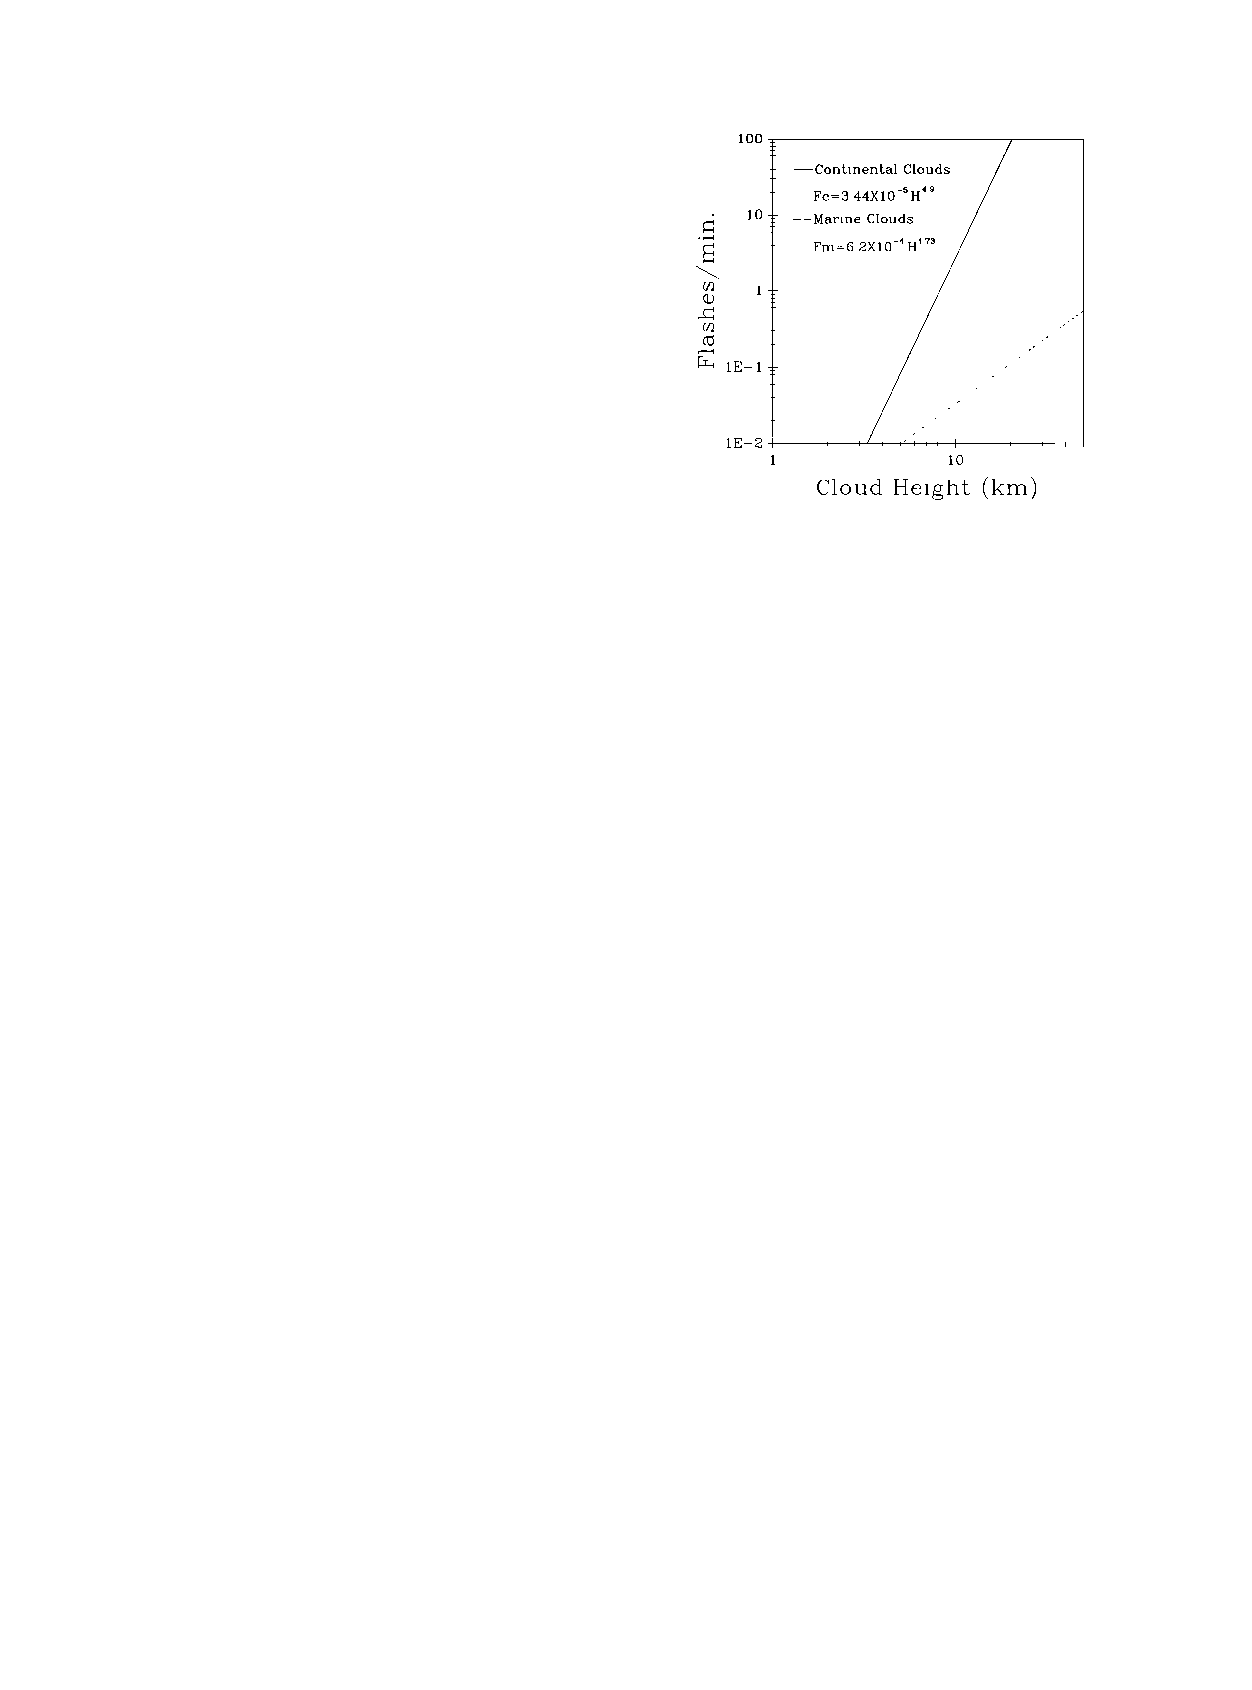
\includegraphics[scale=1]{Price1.pdf} 
   \caption{``Lightning parameterization for continental and maritime thunderstorms" \citep{Price1992}}
   \label{FmFc}
\end{figure}

They used the new relations to redo the lightning frequency using the ISSCP data. A gridbox was considered maritime if there was no land within 500km of any of the edges. So continent was defined as anything within 500km of the coast.

Their lightning satellite only had a 2\% DE, so they made a matched efficiency factor $f$ for each month. They binned up a month of satellite data into a $10^\circ$ x $10^\circ$ grid and found what percentage were below the sensor threshold of 0.2 flashes/min. So if it was 77\% they then created a threshold value for their calculated lightning flash rates so that they threw out bins below that threshold until 77\% were empty.

They then do some statistical tests to see if their predictions (based on 1985? data) matches the observations (based on 1978? data). They also did a comparison in South Africa using the ISCCP data and a count of sferics at the same time.

This leads to a comparison between modern cloud parameters such as cloud top hight, CAPE, and updraft intensity with WWLLN flash rate for an area such as the U.S. or other places. But this {\emph should} have been done by NLDN at some point in the recent past.

\section*{Data Sources}

\citet{Brooks1925} compiled global thunder day data, and based on this came to the estimate of 1800 thunderstorms at a given time assuming that a typical storm lasts 1 hour and has a flash rate of 200 flasher per hour. They also reported that the diurnal pattern of thunderstorm frequency is the same at all latitudes with varying amplitude.

\section*{Variables}

Orography {\bf\citep{Roble1986}}. (from \citet{Siingh2007})

``In fact solar wind, solar flares, galactic cosmic rays, ionospheric�magnetospheric dynamo, thunder cloud, geomagnetic disturbances, solar magnetic sector boundary crossings, solar cycle variations, auroral activity, etc. affect the components of the GEC {\bf\citep{Lakhina1993, Tinsley2000, Singh2004}}" (from \citet{Siingh2007})

\citet{Siingh2007} has an extensive discussion on the variabilities of the GEC from conductivity to solar influences.


\bibliography{/users/michaelhutchins/documents/ess/research/library}
\bibliographystyle{/users/michaelhutchins/documents/ess/research/agu}

\end{document}